\documentclass{beamer}
\usepackage{tikz}
\usepackage{animate}
\usepackage{pgfplots}
\pgfplotsset{compat=1.18}
\usepackage{amsmath}
\usetikzlibrary{graphs, shapes.geometric, positioning}% Enable the shadings library
\usetikzlibrary{backgrounds, fit, shapes.misc, shadows, shapes.symbols}

\usetikzlibrary{shadings}

\usetikzlibrary{ arrows.meta,}
\usepackage{theme/beamer-s4ndm4n}

\usepackage{xcolor}
% \usepackage{helvet} % Use a modern sans-serif font
% \renewcommand{\familydefault}{\sfdefault}
\definecolor{darkblue}{RGB}{0, 71, 171}
\definecolor{lightblue}{RGB}{173, 216, 230}
\definecolor{lightblue2}{RGB}{158, 213, 253}
\definecolor{pblue}{RGB}{117, 154, 254}
\definecolor{greyblue}{RGB}{121, 141, 194}


\title{Protein Language Model}
\author[]{Abony,Sinthia}
\date{28/11/24}

\begin{document}
\usetikzlibrary {shadows}

\begin{frame}[plain]
    \begin{columns}[t]
        % Left column: Full coverage image
        \column{0.5\textwidth}
        \begin{tikzpicture}[remember picture, overlay]
            \node[drop shadow={opacity=1},anchor=north west, inner sep=0, outer sep=0] at (current page.north west) {
                \includegraphics[ height = \paperheight]{images/Screenshot (44)mid1.png} % Adjust the path
            };
        \end{tikzpicture}

        % Right column: Title, author, date
        \column{0.3\textwidth}
        {\Huge \textbf{\textcolor{darkblue}{PML}}} \\[.4cm]
        {\huge \textbf{\textcolor{darkblue}{P}rotein \textcolor{darkblue}{L}anguage \textcolor{darkblue}{M}odel}} \\ [1cm]
        {\textit{Abony Kamal, Mahbuba Sayed Sinthia}} \\[0.5cm]
        {\tiny \today}
    \end{columns}
\end{frame}

\usetikzlibrary{graphs, shapes.geometric, positioning}% Enable the shadings library
\usetikzlibrary{shadings}
\usetikzlibrary {arrows.meta}
\definecolor{vibrantblue}{HTML}{48bfe3}

\begin{frame}
    \frametitle{What is PLM?}
    \begin{center}
        % Main title "PLM"
        \begin{tikzpicture}[remember picture,overlay,node distance=.1mm]
            % Title text
            \node[rectangle,fill=white](org) at (0,0){};
            \node[rectangle, rounded corners, shading=axis, top color=blue!50, bottom color=cyan!20,, align=center, minimum width=10cm,drop shadow, above=1cm of org]
            {A Protein Language Model is a language model\\ that applies the principles of natural language processing \\to predict how proteins fold and function};

            \pause
            \node[circle,left=1.7cm of org, yshift=-1.9cm,,circular glow,outer color=blue!30,inner color=white,, inner sep=0pt](seq){ \includegraphics[width = 3.2cm]{images/sequence.png}};
            \pause
            \node[circle,right=1.7cm of org, yshift=-2cm,circular glow,outer color=purple!30,inner color=white,, inner sep=0pt](struct){ \includegraphics[width = 3.2cm]{images/structprot2.png}};
            \pause
            \node[below=.05cm of org,draw, shading=axis, left color=blue!30, right color=purple!30, text centered, rounded corners, minimum height=3.5cm, minimum width=1.8cm](plm){\textbf{PLM}};

            \draw [red, arrows = {-Stealth[color=blue]}] (seq) to [yshift=-15pt](plm);
             \draw[red, arrows = {-Stealth[color=blue]}] (plm) to [yshift=10pt](struct);

            % % Subtitles with matching colored initials
            % \node[font=\large\bfseries, text=black] at (0, 0.5) {\textcolor{darkblue}{P}ROTEIN};
            % \node[font=\large\bfseries, text=black] at (0, -0.5) {\textcolor{darkblue}{L}ANGUAGE};
            % \node[font=\large\bfseries, text=black] at (0, -1.5) {\textcolor{darkblue}{M}ODEL};
        \end{tikzpicture}
    \end{center}
\end{frame}



\begin{frame}
    \frametitle{What are Language Models?}
    \begin{center}
        % Title block
        
\begin{tikzpicture}
            \node[ text=darkblue, align=center] at (0, 2) {Language Models (LMs)};
        \end{tikzpicture}

        % Explanation in bullet points
        \vspace{0.5cm}
        \begin{itemize}
            \item A language model is a tool that helps computers understand and process human language by learning patterns in large amounts of text.
            % \item It predicts the next word or part of a sentence based on the context, which is useful for tasks like translating languages, answering questions, and generating text.
            \item They are widely used in Natural Language Processing (NLP)
            \item They are used in applications ranging from simple text predictions to complex tasks like machine translation and question answering.
        \end{itemize}

        % Visual representation of text prediction
        % \vspace{1cm}
        % \begin{tikzpicture}
        %     % Input sentence
        %     \node[draw, fill=lightblue!50, rounded corners, text=black,align=center] (input) at (-3, 0) {Input: \\ "I love programming \\ with"};
            
        %     % Arrow
        %     \draw[->, thick, darkblue] (input) -- (2.6, 0) node[midway, above] {Language Model};

        %     % Output words
        %     \node[draw, fill=lightblue!50, rounded corners, text=black, align=center] (output) at (4, 0) {Output: \\ "Python" \\ "JavaScript" \\ "Java"};
        % \end{tikzpicture}
    \end{center}
\end{frame}

\begin{frame}
    \frametitle{How a Language Model Works}

    \begin{columns}
        % Left Column: Bullet Points
        \column{0.5\textwidth}
        \begin{itemize}
            \item <1-> Input Sentence: The model receives a sentence.
            \item <2-> Tokenization: The sentence is broken into tokens (words/subwords).
            \item <3-> Transformer: Tokens are processed by the transformer for context and relationships.
            \item <4-> Prediction: The model predicts the next word.
            \item <5-> Training: The model improves over time through repeated predictions and learning.
        \end{itemize}

        % Right Column: Flow Diagram
        \column{0.5\textwidth}
        \begin{center}
            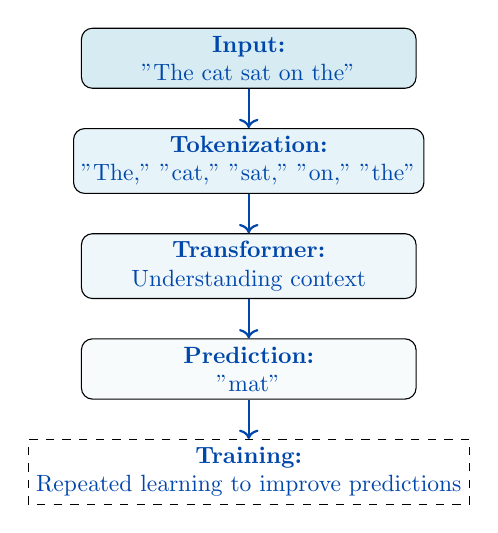
\begin{tikzpicture}[scale=0.7, every node/.style={scale=0.85}]
                % Input Sentence
                \visible<1->{
                    \node[draw, fill=lightblue!50, rounded corners, text=darkblue, align=center, minimum width=5cm] (input) at (0, 2) {
                        \textbf{Input:} \\
                        "The cat sat on the"
                    };
                }

                % Tokenization
                \visible<2->{
                    \node[draw, fill=lightblue!30, rounded corners, text=darkblue, align=center, minimum width=5cm, below=0.5cm of input] (tokenize) {
                        \textbf{Tokenization:} \\
                        "The," "cat," "sat," "on," "the"
                    };
                }

                % Transformer
                \visible<3->{
                    \node[draw, fill=lightblue!20, rounded corners, text=darkblue, align=center, minimum width=5cm, below=0.5cm of tokenize] (transformer) {
                        \textbf{Transformer:} \\
                        Understanding context
                    };
                }

                % Prediction
                \visible<4->{
                    \node[draw, fill=lightblue!10, rounded corners, text=darkblue, align=center, minimum width=5cm, below=0.5cm of transformer] (prediction) {
                        \textbf{Prediction:} \\
                        "mat"
                    };
                }

                % Training
                \visible<5->{
                    \node[draw, dashed, fill=white, text=darkblue, align=center, minimum width=6cm, below=0.5cm of prediction] (training) {
                        \textbf{Training:} \\
                        Repeated learning to improve predictions
                    };
                }
                % Arrows
                \visible<2->{
                    \draw[->, thick, darkblue] (input.south) -- (tokenize.north);
                }
                \visible<3->{
                     \draw[->, thick, darkblue] (tokenize.south) -- (transformer.north);
                }
                \visible<4->{
                     \draw[->, thick, darkblue] (transformer.south) -- (prediction.north);
                }
                \visible<5->{
                    \draw[->, thick, darkblue] (prediction.south) -- (training.north);
                }
                
               
               
                
            \end{tikzpicture}
        \end{center}
    \end{columns}
\end{frame}

\usetikzlibrary{calc}
\usetikzlibrary{positioning}
\usetikzlibrary{fit}

\begin{frame}
    \frametitle{The Language of Proteins}

    \begin{columns}
        % Left Column: Bullet Points
        \column{0.5\textwidth}
        \begin{itemize}
            \item <1-> Proteins are made of \textbf{amino acid sequences} (primary structure) that form the "words" of their language.
            \item <2-> These sequences govern how they fold into shapes (secondary and tertiary structures) that determine their functions.
            \item <3-> Protein language has rules ("grammar") that dictate folding and functionality.
        \end{itemize}

        % Right Column: Flow Chart
        \column{0.5\textwidth}
        \begin{center}
            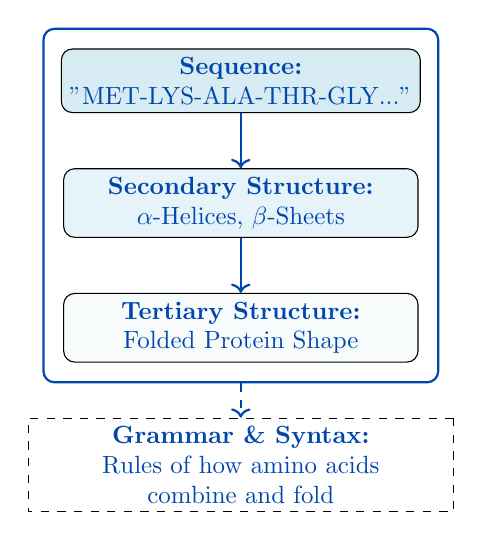
\begin{tikzpicture}[scale=0.9, every node/.style={scale=0.9}]
                % Amino acid sequence block
                \visible<1->{
                    \node[draw, fill=lightblue!50, rounded corners, text=darkblue, align=center, minimum width=5cm] (sequence) at (0, 3) {
                        \textbf{Sequence:} \\ 
                        "MET-LYS-ALA-THR-GLY..."
                    };
                }
                % Secondary structure block
                \visible<2->{
                    \node[draw, fill=lightblue!30, rounded corners, text=darkblue, align=center, minimum width=5cm, below=.7cm of sequence] (secondary) {
                        \textbf{Secondary Structure:} \\
                        $\alpha$-Helices, $\beta$-Sheets
                    };
                }
                % Tertiary structure block
                \visible<2->{
                    \node[draw, fill=lightblue!10, rounded corners, text=darkblue, align=center, minimum width=5cm, below=.7cm of secondary] (tertiary) {
                        \textbf{Tertiary Structure:} \\
                        Folded Protein Shape
                    };
                }
                 % Grammar and Syntax
                 \visible<3->{
                    \node[draw, dashed, fill=white, text=darkblue,align=center, minimum width=6cm, below=.7cm of tertiary] (grammar){
                        \textbf{Grammar \& Syntax:} \\
                        Rules of how amino acids\\ combine and fold
                    };
                }
                % Rounded rectangle around the first three nodes
                % \begin{scope}[visible on=<3->]
                %     \draw[rounded corners, thick, darkblue]
                %         ($(sequence.north west) + (-0.5, 0.3)$) rectangle 
                %         ($(tertiary.south east) + (0.5, -0.3)$);

                % \end{scope}
                \visible<3->{
                    \begin{scope}[]
                        \node[draw, rounded corners, thick, darkblue, fit=(sequence) (tertiary), inner sep=0.5cm] (rect) {};
                    \end{scope}
                }
                % Connections (arrows)
                \visible<2->{
                    \draw[->, thick, darkblue] (sequence.south) -- (secondary.north);
                }
                \visible<2->{
                    \draw[->, thick, darkblue] (secondary.south) -- (tertiary.north);
                }
                \visible<3->{
                    \draw[->, thick, dashed, darkblue] (rect.south) -- (grammar.north);
                }

                
            \end{tikzpicture}
        \end{center}
    \end{columns}
\end{frame}

\begin{frame}
    \frametitle{Parallels of NLP and PLM}

    \begin{columns}
        % Left Column
        \column{0.5\textwidth}
        \begin{center}
            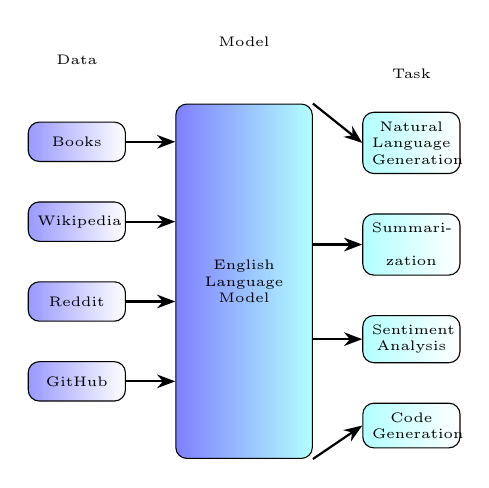
\begin{tikzpicture}[
                node distance=0.3cm and 1.2cm, % Further reduced node distance
                align=center,
                rounded corners,
                every node/.style={font=\tiny}, % Reduced font size
                input/.style={draw,  shading=axis, left color=blue!40, right color=white!30, text width=1cm, minimum height=0.5cm}, % Reduced width and height
                model/.style={draw, shading=axis, left color=blue!50, right color=cyan!30, text width=1.5cm, minimum height=4.5cm, align=center}, % Reduced model node height
                output/.style={draw,   shading=axis, left color=cyan!30, right color=white!30,, text width=1cm, minimum height=0.5cm}, % Reduced width
                arrow/.style={-Stealth, thick},
                scale=0.8 % Scaled down the whole diagram
            ]

            % Input nodes (vertically aligned with equal spacing)
            \visible<2->{
                \node[input] (books) {Books};
                }
            \visible<2->{
                \node[input, below=0.5cm of books] (wikipedia) {Wikipedia};
                }
            \visible<2->{
                \node[input, below=0.5cm of wikipedia] (reddit) {Reddit};
                }
            \visible<2->{
                \node[input, below=0.5cm of reddit] (github) {GitHub};
                }            

            % Model node (with taller height)
            \visible<1->{
                 \node[model, right=1.5cm of wikipedia.south east, yshift=-0.5cm, anchor=center] (model) {English\\ Language\\ Model};
                }
           

            % Output nodes (vertically aligned with equal spacing)
            \visible<3->{
                \node[output, right=1.5cm of model.north, yshift=-.5cm] (nlg) {Natural Language\\ Generation};
                \node[output, below=0.5cm of nlg] (summ) {Summari-\\zation};
                \node[output, below=0.5cm of summ] (sentiment) {Sentiment\\ Analysis};
                \node[output, below=0.5cm of sentiment] (codegen) {Code\\ Generation};
                }
            

            % Headings for sections
            \visible<2->{
                \node[above=0.3cm of books, yshift=0.3cm] {Data}; % Above inputs
                }
            \visible<1->{
                 \node[above=0.3cm of model, yshift=0.3cm] {Model}; % Above model
                }
            \visible<3->{
                 \node[above=0.3cm of nlg] {Task}; % Above outputs

                }

           
 
            % Arrows from inputs to model
            \visible<2->{
                \draw[arrow] (books.east) -- (model.west |- books.east);
                \draw[arrow] (wikipedia.east) -- (model.west |- wikipedia.east);
                \draw[arrow] (reddit.east) -- (model.west |- reddit.east);
                \draw[arrow] (github.east) -- (model.west |- github.east);
                }
            

            % Arrows from model to outputs
            \visible<3->{
                \draw[arrow] (model.north east) -- (nlg.west);
                \draw[arrow] (model.east |- summ.west) -- (summ.west);
                \draw[arrow] (model.east |- sentiment.west) -- (sentiment.west);
                \draw[arrow] (model.south east) -- (codegen.west);
                }
            

            \end{tikzpicture}
        \end{center}

        % Right Column (Duplicate for customization)
        \column{0.5\textwidth}
        \begin{center}
            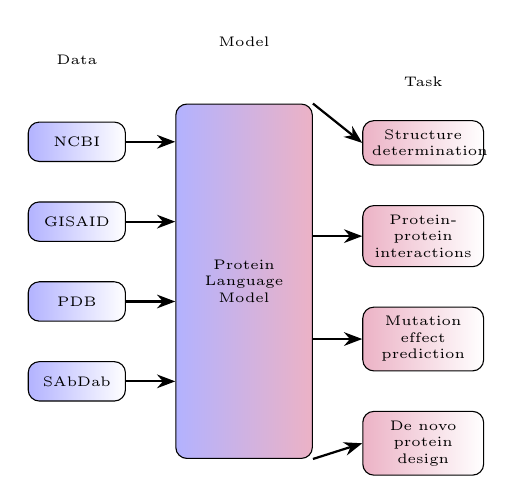
\begin{tikzpicture}[
                node distance=0.3cm and 1.2cm, % Further reduced node distance
                align=center,
                rounded corners,
                every node/.style={font=\tiny}, % Reduced font size
                input/.style={draw,   shading=axis, left color=blue!30, right color=white!30,, text width=1cm, minimum height=0.5cm}, % Reduced width and height
                model/.style={draw, shading=axis, left color=blue!30, right color=purple!30, text width=1.5cm, minimum height=4.5cm, align=center}, % Reduced model node height
                output/.style={draw,  shading=axis, left color=purple!30, right color=white!30,, text width=1.3cm, minimum height=0.5cm}, % Reduced width
                arrow/.style={-Stealth, thick},
                scale=0.8 % Scaled down the whole diagram
            ]

            % Input nodes (vertically aligned with equal spacing)
            \visible<4->{
                 \node[input] (books) {NCBI};
                \node[input, below=0.5cm of books] (wikipedia) {GISAID};
                \node[input, below=0.5cm of wikipedia] (reddit) {PDB};
                \node[input, below=0.5cm of reddit] (github) {SAbDab};
                }
           

            % Model node (with taller height)
            \visible<1->{
                \node[model, right=1.5cm of wikipedia.south east, yshift=-0.5cm, anchor=center] (model) {Protein\\ Language\\ Model};
                }
            

            % Output nodes (vertically aligned with equal spacing)
            \visible<5->{
                \node[output, right=1.5cm of model.north, yshift=-.5cm] (nlg) {Structure\\ determination};
                \node[output, below=0.5cm of nlg] (summ) {Protein-\\protein\\interactions};
                \node[output, below=0.5cm of summ] (sentiment) {Mutation\\ effect\\prediction};
                \node[output, below=0.5cm of sentiment] (codegen) {De novo\\ protein\\design};
                }
            
             % Headings for sections
            \visible<2->{
                \node[above=0.3cm of books, yshift=0.3cm] {Data}; % Above inputs
                }
            \visible<1->{
                 \node[above=0.3cm of model, yshift=0.3cm] {Model}; % Above model
                }
            \visible<3->{
                 \node[above=0.3cm of nlg] {Task}; % Above outputs

                }

            \visible<4->{
                \draw[arrow] (books.east) -- (model.west |- books.east);
                \draw[arrow] (wikipedia.east) -- (model.west |- wikipedia.east);
                \draw[arrow] (reddit.east) -- (model.west |- reddit.east);
                \draw[arrow] (github.east) -- (model.west |- github.east);
                }

            % Arrows from model to outputs
             \visible<5->{
                \draw[arrow] (model.north east) -- (nlg.west);
                \draw[arrow] (model.east |- summ.west) -- (summ.west);
                \draw[arrow] (model.east |- sentiment.west) -- (sentiment.west);
                \draw[arrow] (model.south east) -- (codegen.west);
                }

            \end{tikzpicture}
        \end{center}
    \end{columns}
\end{frame}


\begin{frame}
    \frametitle{Task-Specific Protein Language Models}
    \begin{columns}
        % Left Column: Tasks
        \column{0.45\textwidth}

        \begin{center}
            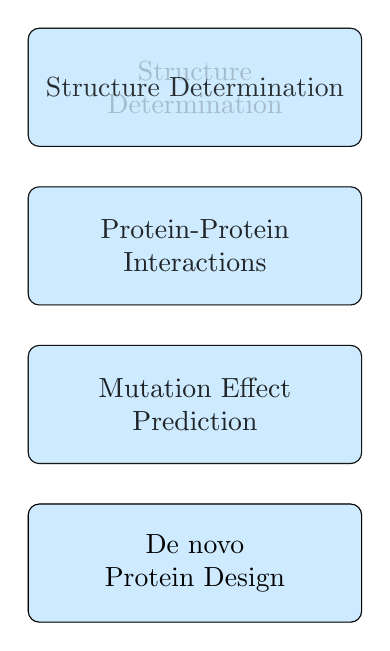
\begin{tikzpicture}[
                node distance=0.3cm and 1.2cm,
                align=center,
                rounded corners,
                every node/.style={},
                input/.style={draw, fill=lightblue2!50, text width=4cm, minimum height=1.5cm},
                arrow/.style={-Stealth, thick},
                scale=0.8
            ]

            % Tasks
            \visible<1>{\node[input, opacity=1] (structure) {Structure Determination};}
            \visible<2->{\node[input, opacity=.2] (structure) {Structure\\ Determination};}
            
            \visible<2>{\node[input, below=0.5cm of structure, opacity=1] (interactions) {Protein-Protein\\Interactions};}
            \visible<1, 3->{\node[input, below=0.5cm of structure, opacity=.2] (interactions) {Protein-Protein\\Interactions};}
            
            \visible<3>{\node[input, below=0.5cm of interactions, opacity=1] (mutation) {Mutation Effect\\ Prediction};}
            \visible<1-2,4->{\node[input, below=0.5cm of interactions, opacity=.2] (mutation) {Mutation Effect\\ Prediction};}
            
            \visible<1-3>{\node[input, below=0.5cm of mutation, opacity=.2] (design) {De novo\\ Protein Design};}
            \visible<4>{\node[input, below=0.5cm of mutation, opacity=1] (design) {De novo\\ Protein Design};}

        \end{tikzpicture}
        \end{center}

        % Right Column: Models
        \column{0.55\textwidth}
        \begin{center}
            \begin{tikzpicture}[
                node distance=0.3cm and 1,
                align=center,
                rounded corners,
                every node/.style={},
                input/.style={draw, fill=greyblue!40, text width=4cm, minimum height=.8cm},
                output/.style={draw,fill=white!10, text width=5cm, minimum height=.8cm},
                arrow/.style={-Stealth, thick},
                scale=0.8
            ]
            \only<1>{
                % \node {\includegraphics[width=\textwidth]{images/stdetr.png}};
                \node[input,text=black](alph) at (0,3.5)
                {AlphaFold};
                \node[below=.25cm of alph](alpic) {\includegraphics[width=5cm, keepaspectratio]{images/stdetr.png}};
                 \node[below=.25cm of alpic] at (alpic.south)
                {Aids in drug discovery, understanding\\ disease mechanisms and designing\\ therapeutic proteins};
            }
             \only<2>{
                \node[input,text=black](ppi) at (0,3.5)
                {DeepPPI};
                \node[below=.25cm of ppi](pipic) {\includegraphics[width=5cm, keepaspectratio]{images/ppi.png}};
                 \node[below=.25cm of pipic] at (pipic.south)
                {Predicts how pathogen proteins\\ interact with human proteins,\\ guiding antiviral/antibacterial \\drug development};
            }
            \only<3>{
                \node[input,text=black](eve) at (0,3.5)
                {EVE \\(Evolutionary Model of Variant Effect Prediction)};
               \node[below=.25cm of eve] (mutpic) {\includegraphics[width=5cm, keepaspectratio]{images/mutation2.png}};
                \node[below=.25cm of mutpic] at (mutpic.south)
                {Predicts whether genetic mutations \\are likely to be disease-causing.};        
            }
             \only<4>{
                % \node {\includegraphics[width=\textwidth]{images/dnovo.png}};
                \node[input,text=black](rose) at (0,3.5)
                {RoseTTAFold};
               \node[below=.25cm of rose] (rosepic) {\includegraphics[width=5cm, keepaspectratio]{images/dnovo.png}};
                \node[below=.25cm of rosepic] at (rosepic.south)
                {Enables the design of novel proteins\\ for industrial applications like\\ biofuels, sustainable materials, and \\green chemistry.};  
            }
            

        \end{tikzpicture}
        \end{center}
    \end{columns}
\end{frame}




\begin{frame}{AlphaFold: Revolutionizing Protein Structure Prediction}
\setbeamercovered{transparent}
    \begin{columns}
        % Left column for text
        \column{0.6\textwidth}
        % \textbf{Overview}
        % \vspace{0.5em}
        \begin{itemize}
            \only<1>{
            \item \textbf{AlphaFold} is an AI model by DeepMind that predicts protein structures with high accuracy.
            }
            \only<2>{
            \item AlphaFold solved a problem that has eluded scientists for decades – predicting a protein's 3D structure from its amino acid sequence.
            \item It achieved \textbf{near-experimental accuracy} in the 2020 CASP competition.
            }
        \end{itemize}
        
        % Right column for images
        \column{0.4\textwidth}
        \begin{center}
            \only<1>{\includegraphics[width=\textwidth]{images/alphafold.png} \\ }
            \vspace{1em}
            \only<2>{\includegraphics[width=\textwidth]{images/graph2-removebg-preview.png} }
        \end{center}
    \end{columns}
\end{frame}

\usetikzlibrary{positioning,shapes.geometric,backgrounds}
\usetikzlibrary{fit}
\usetikzlibrary {shapes.misc}

\usetikzlibrary {shadows,shapes.symbols}

\definecolor{color1}{HTML}{007FFF} % Blue
\definecolor{color2}{HTML}{FF7F00} % Orange
\definecolor{color3}{HTML}{FFD700} % Yellow
\definecolor{color4}{HTML}{00FF00} % Green
\definecolor{color5}{HTML}{FF0000} % Red
\definecolor{color6}{HTML}{FFC0CB} % Pink


% Define shades of orange for similarity matrix
\definecolor{pshade1}{HTML}{FADCD9} % Lightest pink
\definecolor{pshade2}{HTML}{F5A9B8} % Light pink
\definecolor{pshade3}{HTML}{ff9ec2} % Medium pink
\definecolor{pshade4}{HTML}{F06292} % Strong pink
\definecolor{pshade5}{HTML}{E91E63} % Bold pink
\definecolor{pshade6}{HTML}{C2185B} % Darkest pink

% Define shades of orange for similarity matrix
\definecolor{shade1}{HTML}{FFEBCC} % Lightest orange
\definecolor{shade2}{HTML}{FFC266} % Light orange
\definecolor{shade3}{HTML}{FF9933} % Medium orange
\definecolor{shade4}{HTML}{FF6600} % Dark orange
\definecolor{shade5}{HTML}{CC5200} % Darker orange
\definecolor{shade6}{HTML}{993D00} % Darkest orange

\begin{frame}{AlphaFold}
\begin{tikzpicture}[remember picture,overlay,node distance=.1mm]

    %input sequence
    \node[draw, fill=color4, minimum size=1mm] (input_top1) at (0,-1){};
    \node[draw, fill=color6, minimum size=1mm, right=.1mm of input_top1] (input_top2)  {};
    \node[draw, fill=color3, minimum size=1mm, right=.1mm of input_top2] (input_top3) {};
    \node[draw, fill=color2, minimum size=1mm, right=.1mm of input_top3] (input_top4) {};
    \node[draw, fill=color5, minimum size=1mm, right=.1mm of input_top4] (input_top5) {};
    \node[draw, fill=color1, minimum size=1mm, right=.1mm of input_top5] (input_top6) {};
    
    %input sequence label 
    \node[above=.3mm of input_top3,font=\tiny] (input_top_label) {{Input Sequence}};
     %input sequence surrounding box
    \begin{scope}[on background layer]
        \node [draw,bottom color=cyan!20,top color=blue!30,fit=(input_top1)(input_top2)(input_top3)(input_top4)(input_top5)(input_top6) (input_top_label)] (box){};
    \end{scope}

    %%%%%%%%%%%%%%%%%%%%%%%%%%%%%%%%%%%%%%%%%%%%%%%%%%%%%%%%%%%%%%%%%%%%%%%%%%%%%%%%%%%%%
     \visible<5->{
    %pairing
    \node[draw, fill=lightblue, minimum width=1cm, right=.5cm of box,font=\tiny, ] (pair) {Pairing};
    %Generative\\database\\search
    }
    %%%%%%%%%%%%%%%%%%%%%%%%%%%%%%%%%%%%%%%%%%%%%%%%%%%%%%%%%%%%%%%%%%%
    % \node[draw, fill=orange!30, minimum width=1cm, above=2.3cm of pair,font=\tiny,align=center] (db) {Generative\\database\\search};
    \visible<2->{
    \node[draw, above=2.3cm of pair] (db) {\includegraphics[width=1cm]{images/db.png}};
     \node [below=1mm of db,font=\tiny, align=center] {Generative\\database\\search};
    }
    %%%%%%%%%%%%%%%%%%%%%%%%%%%%%%%%%%%%%%%%%%%%%%%%%%%%%%%%%%%%%%%%%%%%%
     \visible<6->{
    %Structural\\database\\search
    % \node[draw, fill=orange!30, minimum width=1cm, below=2cm of pair,font=\tiny,align=center] (sdb) {Structural\\database\\search};
    \node[draw,below=1.5cm of pair] (sdb) {\includegraphics[width=1cm]{images/db.png}};
    \node [below=1mm of sdb,font=\tiny, align=center] {Structural\\database\\search};
    }

     \visible<3->{
    %MSA %%%%%%%%%%%%%%%%%%%%%%%%%%%%%%
     % Input Row
        
        \node[draw, fill=color4, minimum size=1mm, right=1.9cm of db, yshift=1cm] (msa1){};
        \foreach \i/\col/\k in {1/color6/2, 2/color3/3, 3/color2/4, 4/color5/5, 5/color1/6} {
            \node[draw, fill=\col, minimum size=1mm, right=.1mm of msa\i] (msa\k){};
        }

        
        % spcies a
        \node[draw, fill=color5, minimum size=1mm, below=.1mm of msa1] (a1){};
        \foreach \i/\col/\k in {1/color1/2, 2/color4/3, 3/color3/4, 4/color6/5, 5/color2/6} {
            \node[draw, fill=\col, minimum size=1mm, right=.1mm of a\i] (a\k){};
        }
         % spcies b
        \node[draw, fill=color3, minimum size=1mm, below=.1mm of a1] (b1){};
        \foreach \i/\col/\k in {1/color4/2, 2/color2/3, 3/color5/4, 4/color1/5, 5/color6/6} {
            \node[draw, fill=\col, minimum size=1mm, right=.1mm of b\i] (b\k){};
        }
          % spcies c
        \node[draw, fill=color6, minimum size=1mm, below=.1mm of b1] (c1){};
        \foreach \i/\col/\k in {1/color3/2, 2/color5/3, 3/color1/4, 4/color2/5, 5/color4/6} {
            \node[draw, fill=\col, minimum size=1mm, right=.1mm of c\i] (c\k){};
        }
          % spcies d
        \node[draw, fill=color4, minimum size=1mm, below=.1mm of c1] (d1){};
        \foreach \i/\col/\k in {1/color6/2, 2/color1/3, 3/color2/4, 4/color5/5, 5/color6/6} {
            \node[draw, fill=\col, minimum size=1mm, right=.1mm of d\i] (d\k){};
        }
          % spcies e
        \node[draw, fill=color2, minimum size=1mm, below=.1mm of d1] (e1){};
        \foreach \i/\col/\k in {1/color5/2, 2/color4/3, 3/color6/4, 4/color3/5, 5/color1/6} {
            \node[draw, fill=\col, minimum size=1mm, right=.1mm of e\i] (e\k){};
        }
        %labels
        \node [left=.15mm of msa1,font=\tiny] {\textbf{Input}};
        \node [left=.15mm of a1,font=\tiny] {\textbf{species A}};
        \node [left=.15mm of b1,font=\tiny] {\textbf{species B}};
        \node [left=.15mm of c1,font=\tiny](lc1) {\textbf{species C}};
        \node [left=.15mm of d1,font=\tiny] {\textbf{species D}};
        \node [left=.15mm of e1,font=\tiny](sce) {\textbf{species E}};

         \node [below=1mm of sce,font=\tiny, xshift=1.3cm, align=center, yshift=.5mm] {\textbf{Multiple Sequence}\\ \textbf{Alignment(MSA)}};

         }

          \visible<5->{
%%%%%%%%%%Pair alignment%%%%%%%%%%%%%%%%%%%%%%%%%%%%%%%%%%%%%%%%%%%%%%
        % Input Row
        \node[draw, fill=color4, minimum size=1mm, right=1.9cm of pair, yshift=1cm] (cell01){};
        \foreach \i/\col/\k in {01/color6/02, 02/color3/03, 03/color2/04, 04/color5/05, 05/color1/06} {
            \node[draw, fill=\col, minimum size=1mm, right=.1mm of cell\i] (cell\k){};
        }
        %alignment matrix
        \foreach \row/\clr/\k in {1/color4/0, 2/color6/1, 3/color3/2, 4/color2/3, 5/color5/4, 6/color1/5} {
            \foreach \col/\clc in {1/color4, 2/color6, 3/color3, 4/color2, 5/color5, 6/color1} {
                % Each cell is divided into two triangles with different colors
                \node[draw, minimum size=1mm, below=.1mm of cell\k\col] (cell\row\col){};
                \begin{scope}[on background layer]
                    \visible<5->{
                    \fill[\clr] (cell\row\col.south west) -- (cell\row\col.south east) -- (cell\row\col.north west) -- cycle;
                    \fill[\clc] (cell\row\col.north west) -- (cell\row\col.south east) -- (cell\row\col.north east) -- cycle;
                    }
                \end{scope}
            }
        }
        %column input row on the left
        \node[draw, fill=color4, minimum size=1mm, left=.1mm of cell11] (cell10){};
        \foreach \i/\col/\k in {10/color6/20, 20/color3/30, 30/color2/40, 40/color5/50, 50/color1/60} {
            \node[draw, fill=\col, minimum size=1mm, below=.1mm of cell\i] (cell\k){};
        }
        %label of pair alignment
        \node (il) [ rotate=90,left=1mm of cell20, font=\tiny] {Input};
        \node () [above=.1mm of cell03, font=\tiny] {Input};
         \node [below=1.5mm of cell60,font=\tiny, xshift=.8cm] {\textbf{Pair alignment}};
        }

     \visible<7->{
        %templates
        % \node[draw, fill=green!30, minimum width=1cm, right=2cm of sdb,font=\tiny,align=center] (templates) {Templates};
        \node[draw, right=1.6cm of sdb] (templates) {\includegraphics[width=1.7cm]{images/structprot3.png}};
        \node [below=1mm of templates,font=\tiny, align=center] {Templates};
    }

    
     \visible<4->{
%%%%%%%%% MSA representation%%%%%%%%%%%%%%%%%%5
         % Input Row
        
        \node[draw, fill=color4, minimum size=1mm, right=1.5cm of msa6] (msap1){};
        \foreach \i/\col/\k in {1/color6/2, 2/color3/3, 3/color2/4, 4/color5/5, 5/color1/6} {
            \node[draw, fill=\col, minimum size=1mm, right=.1mm of msap\i] (msap\k){};
        }

        %row1 color fill input
        \node[fill=pshade6, minimum size=1mm, below=.1mm of msap1] (ma1) {}; 
        \node[fill=pshade1, minimum size=1mm, right=.1mm of ma1](ma2) {}; 
        \node[fill=pshade4, minimum size=1mm, right=.1mm of ma2](ma3){}; 
        \node[fill=pshade3, minimum size=1mm, right=.1mm of ma3] (ma4){};
        \node[fill=pshade2, minimum size=1mm, right=.1mm of ma4] (ma5){}; 
        \node[fill=pshade4, minimum size=1mm, right=.1mm of ma5] (ma6){}; 

        %row2 color fill 
        \node[fill=pshade6, minimum size=1mm,below=.1mm of ma1] (mb1) {}; 
        \node[fill=pshade4, minimum size=1mm, right=.1mm of mb1] (mb2) {}; 
        \node[fill=pshade2, minimum size=1mm, right=.1mm of mb2] (mb3) {}; 
        \node[fill=pshade3, minimum size=1mm, right=.1mm of mb3] (mb4) {};
        \node[fill=pshade6, minimum size=1mm, right=.1mm of mb4] (mb5) {}; 
        \node[fill=pshade5, minimum size=1mm, right=.1mm of mb5] (mb6) {}; 

         %row3 color fill
        \node[fill=pshade4, minimum size=1mm,below=.1mm of mb1] (mc1) {}; 
        \node[fill=pshade3, minimum size=1mm, right=.1mm of mc1] (mc2) {}; 
        \node[fill=pshade1, minimum size=1mm, right=.1mm of mc2] (mc3) {}; 
        \node[fill=pshade2, minimum size=1mm, right=.1mm of mc3] (mc4) {};
        \node[fill=pshade5, minimum size=1mm, right=.1mm of mc4] (mc5) {}; 
        \node[fill=pshade1, minimum size=1mm, right=.1mm of mc5] (mc6) {};

         %row4 color fill
        \node[fill=pshade1, minimum size=1mm,below=.1mm of mc1] (md1) {}; 
        \node[fill=pshade2, minimum size=1mm, right=.1mm of md1] (md2) {}; 
        \node[fill=pshade6, minimum size=1mm, right=.1mm of md2] (md3) {}; 
        \node[fill=pshade3, minimum size=1mm, right=.1mm of md3] (md4) {};
        \node[fill=pshade5, minimum size=1mm, right=.1mm of md4] (md5) {}; 
        \node[fill=pshade4, minimum size=1mm, right=.1mm of md5](md6) {};

        %row5 color fill
        \node[fill=pshade6, minimum size=1mm,below=.1mm of md1] (me1) {}; 
        \node[fill=pshade3, minimum size=1mm, right=.1mm of me1](me2)  {}; 
        \node[fill=pshade1, minimum size=1mm, right=.1mm of me2] (me3) {}; 
        \node[fill=pshade5, minimum size=1mm, right=.1mm of me3] (me4) {};
        \node[fill=pshade2, minimum size=1mm, right=.1mm of me4] (me5) {}; 
        \node[fill=pshade4, minimum size=1mm, right=.1mm of me5](me6) {};

        %row6 color fill
        \node[fill=pshade1, minimum size=1mm,below=.1mm of me1] (mf1) {}; 
        \node[fill=pshade4, minimum size=1mm, right=.1mm of mf1] (mf2) {}; 
        \node[fill=pshade6, minimum size=1mm, right=.1mm of mf2] (mf3) {}; 
        \node[fill=pshade3, minimum size=1mm, right=.1mm of mf3] (mf4){};
        \node[fill=pshade5, minimum size=1mm, right=.1mm of mf4](mf5) {}; 
        \node[fill=pshade6, minimum size=1mm, right=.1mm of mf5] (mf6){};

        %label
        \node [left=.15mm of msap1,font=\tiny] {\textbf{Input}};
        \node [left=.15mm of ma1,font=\tiny] {\textbf{Input}};
        \foreach \i/\col in {b/A, c/B, d/C, e/D, f/E} {
            \node[left=.15mm of m\i1,font=\tiny](lmp\col){\textbf{\col}};
        }
         \node [below=1mm of lmpE,font=\tiny, xshift=.8cm, yshift=.7mm] {\textbf{MSA representation}};
    }

     \visible<8->{
%%%%%%%% pair representation%%%%%%%%%%%%%%%%%%5
        \node[draw, fill=color4, minimum size=1mm, right=1.5cm of cell06] (pr1){};
        \foreach \i/\col/\k in {1/color6/2, 2/color3/3, 3/color2/4, 4/color5/5, 5/color1/6} {
            \node[draw, fill=\col, minimum size=1mm, right=.1mm of pr\i] (pr\k){};
        }

        %row1 color fill input
        \node[fill=shade6, minimum size=1mm, below=.1mm of pr1] (pa1) {}; 
        \node[fill=shade1, minimum size=1mm, right=.1mm of pa1](pa2) {}; 
        \node[fill=shade4, minimum size=1mm, right=.1mm of pa2](pa3){}; 
        \node[fill=shade3, minimum size=1mm, right=.1mm of pa3] (pa4){};
        \node[fill=shade2, minimum size=1mm, right=.1mm of pa4] (pa5){}; 
        \node[fill=shade4, minimum size=1mm, right=.1mm of pa5] (pa6){}; 

        %row2 color fill 
        \node[fill=shade6, minimum size=1mm,below=.1mm of pa1] (pb1) {}; 
        \node[fill=shade4, minimum size=1mm, right=.1mm of pb1] (pb2) {}; 
        \node[fill=shade2, minimum size=1mm, right=.1mm of pb2] (pb3) {}; 
        \node[fill=shade3, minimum size=1mm, right=.1mm of pb3] (pb4) {};
        \node[fill=shade6, minimum size=1mm, right=.1mm of pb4] (pb5) {}; 
        \node[fill=shade5, minimum size=1mm, right=.1mm of pb5] (pb6) {}; 

         %row3 color fill
        \node[fill=shade4, minimum size=1mm,below=.1mm of pb1] (pc1) {}; 
        \node[fill=shade3, minimum size=1mm, right=.1mm of pc1] (pc2) {}; 
        \node[fill=shade1, minimum size=1mm, right=.1mm of pc2] (pc3) {}; 
        \node[fill=shade2, minimum size=1mm, right=.1mm of pc3] (pc4) {};
        \node[fill=shade5, minimum size=1mm, right=.1mm of pc4] (pc5) {}; 
        \node[fill=shade1, minimum size=1mm, right=.1mm of pc5] (pc6) {};

         %row4 color fill
        \node[fill=shade1, minimum size=1mm,below=.1mm of pc1] (pd1) {}; 
        \node[fill=shade2, minimum size=1mm, right=.1mm of pd1] (pd2) {}; 
        \node[fill=shade6, minimum size=1mm, right=.1mm of pd2] (pd3) {}; 
        \node[fill=shade3, minimum size=1mm, right=.1mm of pd3] (pd4) {};
        \node[fill=shade5, minimum size=1mm, right=.1mm of pd4] (pd5) {}; 
        \node[fill=shade4, minimum size=1mm, right=.1mm of pd5](pd6) {};

        %row5 color fill
        \node[fill=shade6, minimum size=1mm,below=.1mm of pd1] (pe1) {}; 
        \node[fill=shade3, minimum size=1mm, right=.1mm of pe1](pe2)  {}; 
        \node[fill=shade1, minimum size=1mm, right=.1mm of pe2] (pe3) {}; 
        \node[fill=shade5, minimum size=1mm, right=.1mm of pe3] (pe4) {};
        \node[fill=shade2, minimum size=1mm, right=.1mm of pe4] (pe5) {}; 
        \node[fill=shade4, minimum size=1mm, right=.1mm of pe5](pe6) {};

        %row6 color fill
        \node[fill=shade1, minimum size=1mm,below=.1mm of pe1] (pf1) {}; 
        \node[fill=shade4, minimum size=1mm, right=.1mm of pf1] (pf2) {}; 
        \node[fill=shade6, minimum size=1mm, right=.1mm of pf2] (pf3) {}; 
        \node[fill=shade3, minimum size=1mm, right=.1mm of pf3] (pf4){};
        \node[fill=shade5, minimum size=1mm, right=.1mm of pf4](pf5) {}; 
        \node[fill=shade6, minimum size=1mm, right=.1mm of pf5] (pf6){};

        %column input row on the left
        \node[draw, fill=color4, minimum size=1mm, left=.1mm of pa1] (pr10){};
        \foreach \i/\col/\k in {10/color6/20, 20/color3/30, 30/color2/40, 40/color5/50, 50/color1/60} {
            \node[draw, fill=\col, minimum size=1mm, below=.1mm of pr\i] (pr\k){};
        }
        %label of pair alignment
        \node (lpr) [ rotate=90,left=1mm of pr20, font=\tiny] {Input};
        \node () [above=.1mm of pr3, font=\tiny, yshift=-1mm] {Input};
        \node [below=1.5mm of pr60,font=\tiny, xshift=.8cm] {\textbf{Pair representation}};
    }


%%%%%%%%%%%%arrows%%%%%%%%%%%%%%55
    \visible<2->{
    \draw [->] (box) to [bend left=45] (db.west);
    }
    \visible<3->{
    \draw [->] (db) to  (lc1);
    }
    \visible<4->{
    \draw [->] (c6) to  (lmpB);
    }
    \visible<5->{
    \draw [->] (box) to  (pair);
    \draw [->] (pair) to  (il);
    }
    \visible<6->{
    \draw [->] (box) to [bend right=45] (sdb.west);
    }
    \visible<7->{
      \draw [->] (sdb) to  (templates);
    }
    \visible<8->{
    \draw [->] (templates) to [bend right=45] (pf3.south);
     \draw [->] (cell36) to  (lpr);
    }


    
    
    
    
    
  
    
   
    
    
\end{tikzpicture}
\end{frame}


\usetikzlibrary{positioning,shapes.geometric,backgrounds}
\usetikzlibrary{fit}
\usetikzlibrary {shapes.misc}

\usetikzlibrary {shadows,shapes.symbols}

\definecolor{color1}{HTML}{007FFF} % Blue
\definecolor{color2}{HTML}{FF7F00} % Orange
\definecolor{color3}{HTML}{FFD700} % Yellow
\definecolor{color4}{HTML}{00FF00} % Green
\definecolor{color5}{HTML}{FF0000} % Red
\definecolor{color6}{HTML}{FFC0CB} % Pink


% Define shades of orange for similarity matrix
\definecolor{pshade1}{HTML}{FADCD9} % Lightest pink
\definecolor{pshade2}{HTML}{F5A9B8} % Light pink
\definecolor{pshade3}{HTML}{ff9ec2} % Medium pink
\definecolor{pshade4}{HTML}{F06292} % Strong pink
\definecolor{pshade5}{HTML}{E91E63} % Bold pink
\definecolor{pshade6}{HTML}{C2185B} % Darkest pink

% Define shades of orange for similarity matrix
\definecolor{shade1}{HTML}{FFEBCC} % Lightest orange
\definecolor{shade2}{HTML}{FFC266} % Light orange
\definecolor{shade3}{HTML}{FF9933} % Medium orange
\definecolor{shade4}{HTML}{FF6600} % Dark orange
\definecolor{shade5}{HTML}{CC5200} % Darker orange
\definecolor{shade6}{HTML}{993D00} % Darkest orange



\begin{frame}{AlphaFold}
\begin{tikzpicture}[remember picture,overlay,node distance=.1mm]
    \node[ minimum size=1mm] (orgs) at (-.05,-.25){};

    \visible<1->{
        %%%%%%%%% MSA representation%%%%%%%%%%%%%%%%%%5
         % Input Row
        
        \node[draw, fill=color4, minimum size=1mm, above=2cm of orgs] (msap1){};
        \foreach \i/\col/\k in {1/color6/2, 2/color3/3, 3/color2/4, 4/color5/5, 5/color1/6} {
            \node[draw, fill=\col, minimum size=1mm, right=.1mm of msap\i] (msap\k){};
        }

        %row1 color fill input
        \node[fill=pshade6, minimum size=1mm, below=.1mm of msap1] (ma1) {}; 
        \node[fill=pshade1, minimum size=1mm, right=.1mm of ma1](ma2) {}; 
        \node[fill=pshade4, minimum size=1mm, right=.1mm of ma2](ma3){}; 
        \node[fill=pshade3, minimum size=1mm, right=.1mm of ma3] (ma4){};
        \node[fill=pshade2, minimum size=1mm, right=.1mm of ma4] (ma5){}; 
        \node[fill=pshade4, minimum size=1mm, right=.1mm of ma5] (ma6){}; 

        %row2 color fill 
        \node[fill=pshade6, minimum size=1mm,below=.1mm of ma1] (mb1) {}; 
        \node[fill=pshade4, minimum size=1mm, right=.1mm of mb1] (mb2) {}; 
        \node[fill=pshade2, minimum size=1mm, right=.1mm of mb2] (mb3) {}; 
        \node[fill=pshade3, minimum size=1mm, right=.1mm of mb3] (mb4) {};
        \node[fill=pshade6, minimum size=1mm, right=.1mm of mb4] (mb5) {}; 
        \node[fill=pshade5, minimum size=1mm, right=.1mm of mb5] (mb6) {}; 

         %row3 color fill
        \node[fill=pshade4, minimum size=1mm,below=.1mm of mb1] (mc1) {}; 
        \node[fill=pshade3, minimum size=1mm, right=.1mm of mc1] (mc2) {}; 
        \node[fill=pshade1, minimum size=1mm, right=.1mm of mc2] (mc3) {}; 
        \node[fill=pshade2, minimum size=1mm, right=.1mm of mc3] (mc4) {};
        \node[fill=pshade5, minimum size=1mm, right=.1mm of mc4] (mc5) {}; 
        \node[fill=pshade1, minimum size=1mm, right=.1mm of mc5] (mc6) {};

         %row4 color fill
        \node[fill=pshade1, minimum size=1mm,below=.1mm of mc1] (md1) {}; 
        \node[fill=pshade2, minimum size=1mm, right=.1mm of md1] (md2) {}; 
        \node[fill=pshade6, minimum size=1mm, right=.1mm of md2] (md3) {}; 
        \node[fill=pshade3, minimum size=1mm, right=.1mm of md3] (md4) {};
        \node[fill=pshade5, minimum size=1mm, right=.1mm of md4] (md5) {}; 
        \node[fill=pshade4, minimum size=1mm, right=.1mm of md5](md6) {};

        %row5 color fill
        \node[fill=pshade6, minimum size=1mm,below=.1mm of md1] (me1) {}; 
        \node[fill=pshade3, minimum size=1mm, right=.1mm of me1](me2)  {}; 
        \node[fill=pshade1, minimum size=1mm, right=.1mm of me2] (me3) {}; 
        \node[fill=pshade5, minimum size=1mm, right=.1mm of me3] (me4) {};
        \node[fill=pshade2, minimum size=1mm, right=.1mm of me4] (me5) {}; 
        \node[fill=pshade4, minimum size=1mm, right=.1mm of me5](me6) {};

        %row6 color fill
        \node[fill=pshade1, minimum size=1mm,below=.1mm of me1] (mf1) {}; 
        \node[fill=pshade4, minimum size=1mm, right=.1mm of mf1] (mf2) {}; 
        \node[fill=pshade6, minimum size=1mm, right=.1mm of mf2] (mf3) {}; 
        \node[fill=pshade3, minimum size=1mm, right=.1mm of mf3] (mf4){};
        \node[fill=pshade5, minimum size=1mm, right=.1mm of mf4](mf5) {}; 
        \node[fill=pshade6, minimum size=1mm, right=.1mm of mf5] (mf6){};

        %label
        \node [left=.15mm of msap1,font=\tiny] {\textbf{Input}};
        \node [left=.15mm of ma1,font=\tiny] {\textbf{Input}};
        \foreach \i/\col in {b/A, c/B, d/C, e/D, f/E} {
            \node[left=.15mm of m\i1,font=\tiny](lmp\col){\textbf{\col}};
        }
        \node [above=.1mm of orgs,font=\tiny, xshift=5.3mm, yshift=-3mm] {\textbf{MSA representation}};
        
        %%%%%%%% pair representation%%%%%%%%%%%%%%%%%%5
        \node[draw, fill=color4, minimum size=1mm, below=.7cm of orgs] (pr1){};
        \foreach \i/\col/\k in {1/color6/2, 2/color3/3, 3/color2/4, 4/color5/5, 5/color1/6} {
            \node[draw, fill=\col, minimum size=1mm, right=.1mm of pr\i] (pr\k){};
        }

        %row1 color fill input
        \node[fill=shade6, minimum size=1mm, below=.1mm of pr1] (pa1) {}; 
        \node[fill=shade1, minimum size=1mm, right=.1mm of pa1](pa2) {}; 
        \node[fill=shade4, minimum size=1mm, right=.1mm of pa2](pa3){}; 
        \node[fill=shade3, minimum size=1mm, right=.1mm of pa3] (pa4){};
        \node[fill=shade2, minimum size=1mm, right=.1mm of pa4] (pa5){}; 
        \node[fill=shade4, minimum size=1mm, right=.1mm of pa5] (pa6){}; 

        %row2 color fill 
        \node[fill=shade6, minimum size=1mm,below=.1mm of pa1] (pb1) {}; 
        \node[fill=shade4, minimum size=1mm, right=.1mm of pb1] (pb2) {}; 
        \node[fill=shade2, minimum size=1mm, right=.1mm of pb2] (pb3) {}; 
        \node[fill=shade3, minimum size=1mm, right=.1mm of pb3] (pb4) {};
        \node[fill=shade6, minimum size=1mm, right=.1mm of pb4] (pb5) {}; 
        \node[fill=shade5, minimum size=1mm, right=.1mm of pb5] (pb6) {}; 

         %row3 color fill
        \node[fill=shade4, minimum size=1mm,below=.1mm of pb1] (pc1) {}; 
        \node[fill=shade3, minimum size=1mm, right=.1mm of pc1] (pc2) {}; 
        \node[fill=shade1, minimum size=1mm, right=.1mm of pc2] (pc3) {}; 
        \node[fill=shade2, minimum size=1mm, right=.1mm of pc3] (pc4) {};
        \node[fill=shade5, minimum size=1mm, right=.1mm of pc4] (pc5) {}; 
        \node[fill=shade1, minimum size=1mm, right=.1mm of pc5] (pc6) {};

         %row4 color fill
        \node[fill=shade1, minimum size=1mm,below=.1mm of pc1] (pd1) {}; 
        \node[fill=shade2, minimum size=1mm, right=.1mm of pd1] (pd2) {}; 
        \node[fill=shade6, minimum size=1mm, right=.1mm of pd2] (pd3) {}; 
        \node[fill=shade3, minimum size=1mm, right=.1mm of pd3] (pd4) {};
        \node[fill=shade5, minimum size=1mm, right=.1mm of pd4] (pd5) {}; 
        \node[fill=shade4, minimum size=1mm, right=.1mm of pd5](pd6) {};

        %row5 color fill
        \node[fill=shade6, minimum size=1mm,below=.1mm of pd1] (pe1) {}; 
        \node[fill=shade3, minimum size=1mm, right=.1mm of pe1](pe2)  {}; 
        \node[fill=shade1, minimum size=1mm, right=.1mm of pe2] (pe3) {}; 
        \node[fill=shade5, minimum size=1mm, right=.1mm of pe3] (pe4) {};
        \node[fill=shade2, minimum size=1mm, right=.1mm of pe4] (pe5) {}; 
        \node[fill=shade4, minimum size=1mm, right=.1mm of pe5](pe6) {};

        %row6 color fill
        \node[fill=shade1, minimum size=1mm,below=.1mm of pe1] (pf1) {}; 
        \node[fill=shade4, minimum size=1mm, right=.1mm of pf1] (pf2) {}; 
        \node[fill=shade6, minimum size=1mm, right=.1mm of pf2] (pf3) {}; 
        \node[fill=shade3, minimum size=1mm, right=.1mm of pf3] (pf4){};
        \node[fill=shade5, minimum size=1mm, right=.1mm of pf4](pf5) {}; 
        \node[fill=shade6, minimum size=1mm, right=.1mm of pf5] (pf6){};

        %column input row on the left
        \node[draw, fill=color4, minimum size=1mm, left=.1mm of pa1] (pr10){};
        \foreach \i/\col/\k in {10/color6/20, 20/color3/30, 30/color2/40, 40/color5/50, 50/color1/60} {
            \node[draw, fill=\col, minimum size=1mm, below=.1mm of pr\i] (pr\k){};
        }
        %label of pair alignment
        \node (lpr) [ rotate=90,left=1mm of pr20, font=\tiny] {Input};
        \node () [above=.1mm of pr3, font=\tiny] {Input};

        \node [below=1.5mm of pr60,font=\tiny, xshift=.8cm] {\textbf{Pair representation}};

    }

    
    \visible<2-6>{
        %%%%%%%%%%%%%%%% evoformer%%%%%%%%%%%%%%%%
        \node[rounded corners,
        double copy shadow={opacity=.5,shadow xshift=1ex,shadow yshift=1ex, left color=blue!20, right color=blue!60},
        draw=blue, left color=blue!20, right color=blue!60, align=center
        ,minimum height=5.7cm, 
        font=\fontsize{8pt}{10pt}\selectfont, 
        right=2.2cm of orgs, yshift=-.2cm]
        (evoformer){\textbf{Evoformer}\\ \\ 48 blocks};
    }

     \only<7->{
        %%%%%%%%%%%%%%%% evoformer%%%%%%%%%%%%%%%%
        \node[rounded corners,
        double copy shadow={opacity=.5,shadow xshift=1ex,shadow yshift=1ex, left color=blue!20, right color=blue!60},
        draw=blue, left color=cyan!30, right color=blue!60, align=center
        ,minimum height=5.7cm, 
        font=\fontsize{8pt}{10pt}\selectfont, 
        right=2.2cm of orgs, yshift=-.2cm]
        (evoformer){\textbf{Evoformer}\\ \\ 48 blocks};
    }

     \visible<3->{
        %%%%%%%%% MSA representation%%%%%%%%%%%%%%%%%%5
         % Input Row
        
        \node[draw, fill=color4, minimum size=1mm, right=3.8cm of msap6] (xmsap1){};
        \foreach \i/\col/\k in {1/color6/2, 2/color3/3, 3/color2/4, 4/color5/5, 5/color1/6} {
            \node[draw, fill=\col, minimum size=1mm, right=.1mm of xmsap\i] (xmsap\k){};
        }

        %row1 color fill input
        \node[fill=pshade6, minimum size=1mm, below=.1mm of xmsap1] (xma1) {}; 
        \node[fill=pshade1, minimum size=1mm, right=.1mm of xma1](xma2) {}; 
        \node[fill=pshade4, minimum size=1mm, right=.1mm of xma2](xma3){}; 
        \node[fill=pshade3, minimum size=1mm, right=.1mm of xma3] (xma4){};
        \node[fill=pshade2, minimum size=1mm, right=.1mm of xma4] (xma5){}; 
        \node[fill=pshade4, minimum size=1mm, right=.1mm of xma5] (xma6){}; 

        %row2 color fill 
        \node[fill=pshade6, minimum size=1mm,below=.1mm of xma1] (xmb1) {}; 
        \node[fill=pshade4, minimum size=1mm, right=.1mm of xmb1] (xmb2) {}; 
        \node[fill=pshade2, minimum size=1mm, right=.1mm of xmb2] (xmb3) {}; 
        \node[fill=pshade3, minimum size=1mm, right=.1mm of xmb3] (xmb4) {};
        \node[fill=pshade6, minimum size=1mm, right=.1mm of xmb4] (xmb5) {}; 
        \node[fill=pshade5, minimum size=1mm, right=.1mm of xmb5] (xmb6) {}; 

         %row3 color fill
        \node[fill=pshade4, minimum size=1mm,below=.1mm of xmb1] (xmc1) {}; 
        \node[fill=pshade3, minimum size=1mm, right=.1mm of xmc1] (xmc2) {}; 
        \node[fill=pshade1, minimum size=1mm, right=.1mm of xmc2] (xmc3) {}; 
        \node[fill=pshade2, minimum size=1mm, right=.1mm of xmc3] (xmc4) {};
        \node[fill=pshade5, minimum size=1mm, right=.1mm of xmc4] (xmc5) {}; 
        \node[fill=pshade1, minimum size=1mm, right=.1mm of xmc5] (xmc6) {};

         %row4 color fill
        \node[fill=pshade1, minimum size=1mm,below=.1mm of xmc1] (xmd1) {}; 
        \node[fill=pshade2, minimum size=1mm, right=.1mm of xmd1] (xmd2) {}; 
        \node[fill=pshade6, minimum size=1mm, right=.1mm of xmd2] (xmd3) {}; 
        \node[fill=pshade3, minimum size=1mm, right=.1mm of xmd3] (xmd4) {};
        \node[fill=pshade5, minimum size=1mm, right=.1mm of xmd4] (xmd5) {}; 
        \node[fill=pshade4, minimum size=1mm, right=.1mm of xmd5](xmd6) {};

        %row5 color fill
        \node[fill=pshade6, minimum size=1mm,below=.1mm of xmd1] (xme1) {}; 
        \node[fill=pshade3, minimum size=1mm, right=.1mm of xme1](xme2)  {}; 
        \node[fill=pshade1, minimum size=1mm, right=.1mm of xme2] (xme3) {}; 
        \node[fill=pshade5, minimum size=1mm, right=.1mm of xme3] (xme4) {};
        \node[fill=pshade2, minimum size=1mm, right=.1mm of xme4] (xme5) {}; 
        \node[fill=pshade4, minimum size=1mm, right=.1mm of xme5](xme6) {};

        %row6 color fill
        \node[fill=pshade1, minimum size=1mm,below=.1mm of xme1] (xmf1) {}; 
        \node[fill=pshade4, minimum size=1mm, right=.1mm of xmf1] (xmf2) {}; 
        \node[fill=pshade6, minimum size=1mm, right=.1mm of xmf2] (xmf3) {}; 
        \node[fill=pshade3, minimum size=1mm, right=.1mm of xmf3] (xmf4){};
        \node[fill=pshade5, minimum size=1mm, right=.1mm of xmf4](xmf5) {}; 
        \node[fill=pshade6, minimum size=1mm, right=.1mm of xmf5] (xmf6){};

        %label
        \node [left=.15mm of xmsap1,font=\tiny] {\textbf{Input}};
        \node [left=.15mm of xma1,font=\tiny] {\textbf{Input}};
        \foreach \i/\col in {b/A, c/B, d/C, e/D, f/E} {
            \node[left=.15mm of xm\i1,font=\tiny](xlmp\col){\textbf{\col}};
        }

        \node [below=1.5mm of xlmpE,font=\tiny, xshift=.8cm] {\textbf{MSA representation}};

        %%%%%%%% pair representation%%%%%%%%%%%%%%%%%%5
        \node[draw, fill=color4, minimum size=1mm, right=3.8cm of pr6] (xpr1){};
        \foreach \i/\col/\k in {1/color6/2, 2/color3/3, 3/color2/4, 4/color5/5, 5/color1/6} {
            \node[draw, fill=\col, minimum size=1mm, right=.1mm of xpr\i] (xpr\k){};
        }

        %row1 color fill input
        \node[fill=shade6, minimum size=1mm, below=.1mm of xpr1] (xpa1) {}; 
        \node[fill=shade1, minimum size=1mm, right=.1mm of xpa1](xpa2) {}; 
        \node[fill=shade4, minimum size=1mm, right=.1mm of xpa2](xpa3){}; 
        \node[fill=shade3, minimum size=1mm, right=.1mm of xpa3] (xpa4){};
        \node[fill=shade2, minimum size=1mm, right=.1mm of xpa4] (xpa5){}; 
        \node[fill=shade4, minimum size=1mm, right=.1mm of xpa5] (xpa6){}; 

        %row2 color fill 
        \node[fill=shade6, minimum size=1mm,below=.1mm of xpa1] (xpb1) {}; 
        \node[fill=shade4, minimum size=1mm, right=.1mm of xpb1] (xpb2) {}; 
        \node[fill=shade2, minimum size=1mm, right=.1mm of xpb2] (xpb3) {}; 
        \node[fill=shade3, minimum size=1mm, right=.1mm of xpb3] (xpb4) {};
        \node[fill=shade6, minimum size=1mm, right=.1mm of xpb4] (xpb5) {}; 
        \node[fill=shade5, minimum size=1mm, right=.1mm of xpb5] (xpb6) {}; 

         %row3 color fill
        \node[fill=shade4, minimum size=1mm,below=.1mm of xpb1] (xpc1) {}; 
        \node[fill=shade3, minimum size=1mm, right=.1mm of xpc1] (xpc2) {}; 
        \node[fill=shade1, minimum size=1mm, right=.1mm of xpc2] (xpc3) {}; 
        \node[fill=shade2, minimum size=1mm, right=.1mm of xpc3] (xpc4) {};
        \node[fill=shade5, minimum size=1mm, right=.1mm of xpc4] (xpc5) {}; 
        \node[fill=shade1, minimum size=1mm, right=.1mm of xpc5] (xpc6) {};

         %row4 color fill
        \node[fill=shade1, minimum size=1mm,below=.1mm of xpc1] (xpd1) {}; 
        \node[fill=shade2, minimum size=1mm, right=.1mm of xpd1] (xpd2) {}; 
        \node[fill=shade6, minimum size=1mm, right=.1mm of xpd2] (xpd3) {}; 
        \node[fill=shade3, minimum size=1mm, right=.1mm of xpd3] (xpd4) {};
        \node[fill=shade5, minimum size=1mm, right=.1mm of xpd4] (xpd5) {}; 
        \node[fill=shade4, minimum size=1mm, right=.1mm of xpd5](xpd6) {};

        %row5 color fill
        \node[fill=shade6, minimum size=1mm,below=.1mm of xpd1] (xpe1) {}; 
        \node[fill=shade3, minimum size=1mm, right=.1mm of xpe1](xpe2)  {}; 
        \node[fill=shade1, minimum size=1mm, right=.1mm of xpe2] (xpe3) {}; 
        \node[fill=shade5, minimum size=1mm, right=.1mm of xpe3] (xpe4) {};
        \node[fill=shade2, minimum size=1mm, right=.1mm of xpe4] (xpe5) {}; 
        \node[fill=shade4, minimum size=1mm, right=.1mm of xpe5](xpe6) {};

        %row6 color fill
        \node[fill=shade1, minimum size=1mm,below=.1mm of xpe1] (xpf1) {}; 
        \node[fill=shade4, minimum size=1mm, right=.1mm of xpf1] (xpf2) {}; 
        \node[fill=shade6, minimum size=1mm, right=.1mm of xpf2] (xpf3) {}; 
        \node[fill=shade3, minimum size=1mm, right=.1mm of xpf3] (xpf4){};
        \node[fill=shade5, minimum size=1mm, right=.1mm of xpf4](xpf5) {}; 
        \node[fill=shade6, minimum size=1mm, right=.1mm of xpf5] (xpf6){};

        %column input row on the left
        \node[draw, fill=color4, minimum size=1mm, left=.1mm of xpa1] (xpr10){};
        \foreach \i/\col/\k in {10/color6/20, 20/color3/30, 30/color2/40, 40/color5/50, 50/color1/60} {
            \node[draw, fill=\col, minimum size=1mm, below=.1mm of xpr\i] (xpr\k){};
        }
        %label of pair alignment
        \node (xlpr) [ rotate=90,left=1mm of xpr20, font=\tiny] {Input};
        \node () [above=.1mm of xpr3, font=\tiny] {Input};

        \node [below=1.5mm of xpr60,font=\tiny, xshift=.8cm] {\textbf{Pair representation}};
    }

     \visible<4-7>{
        %%%%%%%%%%%%%%%% structure module%%%%%%%%%%%%%%%%
        \node[rounded corners,
        double copy shadow={opacity=.5,shadow xshift=.5ex,shadow yshift=.5ex, left color=blue!20, right color=blue!50},
        draw=blue, left color=blue!20, right color=blue!50, align=center
        ,minimum height=5.7cm, 
        font=\tiny, 
        right=7.5cm of orgs, yshift=-.2cm]
        (sm){\textbf{Structure}\\ \textbf{module}\\ \\8 blocks};
    }

    \only<8->{
        %%%%%%%%%%%%%%%% structure module%%%%%%%%%%%%%%%%
        \node[rounded corners,
        double copy shadow={opacity=.5,shadow xshift=.5ex,shadow yshift=.5ex, left color=blue!20, right color=blue!50},
        draw=blue, left color=cyan!30, right color=blue!50, align=center
        ,minimum height=5.7cm, 
        font=\tiny, 
        right=7.5cm of orgs, yshift=-.2cm]
        (sm){\textbf{Structure}\\ \textbf{module}\\ \\8 blocks};
    }

     \visible<5-8>{
        %%%%%%%%%%%%%%%%%%protein%%%%%%%%%%%%%%%%%%%
         % Define the image inside a circular node
        \node[circle,,circular glow,outer color=blue!30,inner color=white, right=9.4cm of orgs, inner sep=0pt] (img) 
        {\includegraphics[width=1.6cm, angle=-90]{images/protein.png}}; 
        \node [below=2mm of img,font=\tiny, align=center] {\textbf{Initial}\\ \textbf{protein}\\ \textbf{structure}};
    }

    \only<9->{
        %%%%%%%%%%%%%%%%%%protein%%%%%%%%%%%%%%%%%%%
         % Define the image inside a circular node
        \node[circle,,circular glow,outer color=cyan!50,inner color=white, right=9.4cm of orgs, inner sep=0pt] (img) 
        {\includegraphics[width=1.6cm, angle=-90]{images/protein.png}}; 
        \node [below=2mm of img,font=\tiny, align=center] {\textbf{Predicted}\\ \textbf{protein}\\ \textbf{structure}};
    }
        % % Add a label below the circle
        % \node[below of=imageNode] (label) {This is the image};

        %%%%%%%%%%%%%%%%%%arrows
        \visible<2->{
             \draw [->] (mc6.east) to  ([yshift=46pt]evoformer.west);
             \draw [->] (pc6.east) to  ([yshift=-46pt]evoformer.west);
         }

         \visible<3->{
            \draw [->] ([yshift=46pt]evoformer.east) to  (xlmpB.west);
            \draw [->] ([yshift=-48pt]evoformer.east) to  (xlpr.north);
         } 
       
         \visible<4->{
            \draw [->] (xmc6.east) to  ([yshift=46pt]sm.west);
            \draw [->] (xpc6.east) to  ([yshift=-46pt]sm.west);
         }

         \visible<5->{
            \draw [->] ([yshift=6pt]sm.east) to  (img.west);
         }
        
         \visible<6-8>{
            \draw [->] (img.south) to [out=-115, in=-30] (pf3.south);
            \draw [->] (img.north) to [out=115, in=30] (msap3.north);
         }

        
        
        

\end{tikzpicture}
\end{frame}
        

\begin{frame}{ProtBERT: A Protein Language Model}
\setbeamercovered{transparent}
    \begin{columns}
        % Left column for text
        \column{0.6\textwidth}
        \textbf{Overview}
        \vspace{0.5em}
        \begin{itemize}
            \item<1> \textbf{ProtBERT} is a pre-trained language model specifically designed for proteins.
            \item<2> It uses a \textbf{transformer architecture} similar to BERT, but adapted for protein sequences.
        \end{itemize}
        
        % Right column for images
        \column{0.4\textwidth}
        \begin{center}
            \only<1>{\includegraphics[width=\textwidth]{images/nucleosome.jpeg} \\ }
            \vspace{1em}
            \only<2>{\includegraphics[width=\textwidth]{images/transformers.PNG} }
        \end{center}
    \end{columns}
\end{frame}


\begin{frame}
    \frametitle{ProtBERT: Key Features}
    \begin{columns}
        % Left Column: Tasks
        \column{0.45\textwidth}

        \begin{center}
            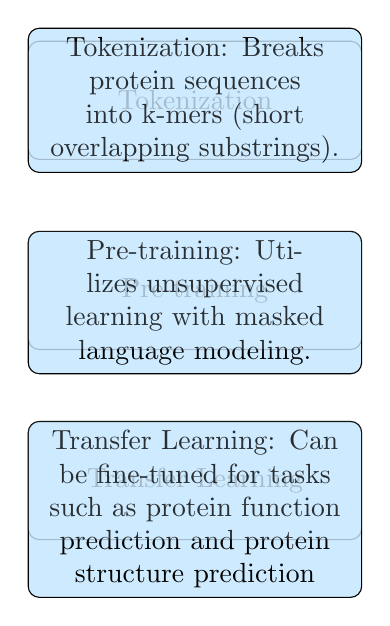
\begin{tikzpicture}[
                node distance=0.3cm and 1.2cm,
                align=center,
                rounded corners,
                every node/.style={},
                input/.style={draw, fill=lightblue2!50, text width=4cm, minimum height=1.5cm},
                arrow/.style={-Stealth, thick},
                scale=0.8
            ]

            % Tasks
            \visible<1>{\node[input, opacity=1] (structure) {Tokenization:
Breaks protein
sequences into
k-mers (short
overlapping
substrings).};}
            \visible<2->{\node[input, opacity=.2] (structure) {Tokenization};}
            
            \visible<2>{\node[input, below=0.9cm of structure, opacity=1] (interactions) {Pre-training:
            Utilizes unsupervised learning with masked language modeling.};}
            \visible<1, 3->{\node[input, below=0.9cm of structure, opacity=.2] (interactions) {Pre-training};}
            
            \visible<3>{\node[input, below=0.9cm of interactions, opacity=1] (mutation) {Transfer Learning: Can be fine-tuned for tasks such as protein function prediction and protein structure prediction};}
            \visible<1-2>{\node[input, below=0.9cm of interactions, opacity=.2] (mutation) {Transfer Learning};}

        \end{tikzpicture}
        \end{center}

        % Right Column: Models
        \column{0.55\textwidth}
        \begin{center}
            \begin{tikzpicture}[
                node distance=0.3cm and 1,
                align=center,
                rounded corners,
                every node/.style={},
                input/.style={draw, fill=greyblue!40, text width=4cm, minimum height=.8cm},
                output/.style={draw,fill=white!10, text width=5cm, minimum height=.8cm},
                arrow/.style={-Stealth, thick},
                scale=0.8
            ]
            \only<1>{
                % \node {\includegraphics[width=\textwidth]{images/stdetr.png}};
                \node[](alpic) at (0,3.5) {\includegraphics[width=3cm, keepaspectratio]{images/K-mer_diagram.svg.png}};
            }
             \only<2>{
                \node[](pipic) at (0,3.5) {\includegraphics[width=5cm, keepaspectratio]{images/pretraining.PNG}};
            }
            \only<3>{
               \node[] (mutpic) at (0,3.5) {\includegraphics[width=7cm, keepaspectratio]{images/transfer_learning.PNG}};
            }
            

        \end{tikzpicture}
        \end{center}
    \end{columns}
\end{frame}





\usetikzlibrary{positioning, shapes.geometric, fit, arrows.meta, patterns}
\usetikzlibrary{overlay-beamer-styles}

\setbeamercovered{transparent}

\begin{frame}{ProtBERT}
    \begin{tikzpicture}[node distance=1cm, every node/.style={font=\small}]
        % Input boxes
        \node[draw, rectangle, fill= blue!20, rounded corners, minimum size=0.5cm, <1->] (s) at (-5, 5) {S};
        \node[draw, rectangle,fill= blue!20, rounded corners, minimum size=0.5cm, visible on=<1->] (e) [right=of s] {E};
        \node[draw, rectangle,fill= blue!20, rounded corners, minimum size=0.5cm, visible on=<1->] (q) [right=of e] {Q};
        \node[draw, rectangle,fill= blue!20, rounded corners, minimum size=0.5cm, visible on=<1->] (dots) [right=of q] {$\dots$};

        % Input text
        \node[align=left, right=2cm of dots, visible on=<1->] (input_text) {Input of \\ length $L$};

        % Striped boxes below the input boxes
        \node[draw, rectangle, pattern=north east lines, minimum size=0.5cm, below = 0.5cm of s, visible on=<2->] (striped1)  {};
        \node[draw, rectangle, pattern=north east lines, minimum size=0.5cm, visible on=<2->] (striped2) [right=of striped1] {};
        \node[draw, rectangle, pattern=north east lines, minimum size=0.5cm, visible on=<2->] (striped3) [right=of striped2] {};
        \node[draw, rectangle, pattern=north east lines, minimum size=0.5cm, visible on=<2->] (striped4) [right=of striped3] {};

        % Tokenization text
        \node[[align=left,below=0.8 cm of input_text, visible on=<2->] (tokenization_text) {Tokenization \\ \& Encoding};

        % Downward arrows
        \draw[->, visible on=<2->] (s) -- (striped1);
        \draw[->, visible on=<2->] (e) -- (striped2);
        \draw[->, visible on=<2->] (q) -- (striped3);
        \draw[->, visible on=<2->] (dots) -- (striped4);
        \draw[->, visible on=<2->] (input_text) -- (tokenization_text)

        % Text on the right of transformer
        \node[ align=center, below=0.5 cm of tokenization_text, visible on=<3->] (attention) 
        {Stack of $N$ \\ self-attention layers};

         % Big rectangle for Transformer model
        \node[draw, rectangle, shading=axis, left color=red!50, right color=blue!30, rounded corners, minimum width=5cm, minimum height=2cm, align=center, left=1.2 cm of attention, visible on=<3->] (transformer) 
        { Transformer Model\\ \rule{5cm}{0.4pt} \\ Last Hidden Layer};

        % Arrows connecting striped boxes and tokenization text
        \draw[->, visible on=<3->] (striped1.south) -- (transformer.north);
        \draw[->, visible on=<3->] (striped2.south) -- (transformer.north);
        \draw[->, visible on=<3->] (striped3.south) -- (transformer.north);
        \draw[->, visible on=<3->] (striped4.south) -- (transformer.north);

        

        \draw[->, visible on=<3->] (tokenization_text) -- (attention)

        % Black boxes below Transformer
        \node[draw, rectangle, fill=black, minimum size=0.2cm, below = 3.5cm of striped1, visible on=<4->] (black1) {};
        \node[draw, rectangle, fill=black, minimum size=0.2cm, below = 3.5cm of striped2, visible on=<4->] (black2) {};
        \node[draw, rectangle, fill=black, minimum size=0.2cm, below = 3.5cm of striped3, visible on=<4->] (black3) {};
        \node[draw, rectangle, fill=black, minimum size=0.2cm, below = 3.5cm of striped4, visible on=<4->] (black4) {};

        % Text "1024" over black boxes
        \node[above=0.1cm of black1, visible on=<4->] {1024};
        \node[above=0.1cm of black2, visible on=<4->] {1024};
        \node[above=0.1cm of black3, visible on=<4->] {1024};
        \node[above=0.1cm of black4, visible on=<4->] {1024};

        % Black box connections
        \draw[->, visible on=<4->] (transformer.south) --  (black1.north);
        \draw[->, visible on=<4->] (transformer.south) --  (black2.north);
        \draw[->, visible on=<4->] (transformer.south) --  (black3.north);
        \draw[->, visible on=<4->] (transformer.south) --  (black4.north);

        % Text "L amino-acid embeddings" on the right
        \node[right=2.6cm of black3, visible on=<4->] (amino) {L amino-acid embeddings};

        \draw[->, visible on=<4->] (attention) -- (amino);

        % Supervised Network text
        \node[below=0.5cm of amino, visible on=<5->] (supervised) {Supervised Network};

        \draw[->, visible on=<5->] (amino) -- (supervised)

        % CNN layer below black boxes
        \node[draw, rectangle,shading=axis, left color=green!50, right color=cyan!30, rounded corners, minimum width=5cm, minimum height=0.5cm, align=center, left = 1.2 cm of supervised, visible on=<5->] 
        (cnn)  {CNN};

        

        % Little rectangles below CNN
        \node[draw, rectangle,fill= orange!20, rounded corners, minimum size=0.5cm, below = 2cm of black1, visible on=<6->] (h1){H};
        \node[draw, rectangle,fill= orange!20, rounded corners, minimum size=0.5cm, right=1cm of h1, visible on=<6->] (h2) {H};
        \node[draw, rectangle,fill= orange!20, rounded corners, minimum size=0.5cm, right=1cm of h2, visible on=<6->] (e) {E};
        \node[draw, rectangle,fill= orange!20, rounded corners, minimum size=0.5cm, right=1cm of e, visible on=<6->] (dots2) {$\dots$};

        % Text "Token-level classification" on the right
        \node[right=0.8cm of dots2, visible on=<6->] (classification) {Token-level classification};

        % Arrows from black boxes to CNN
        \draw[->, visible on=<5->] (black1.south) --  (cnn.north);
        \draw[->, visible on=<5->] (black2.south) --  (cnn.north);
        \draw[->, visible on=<5->] (black3.south) --  (cnn.north);
        \draw[->, visible on=<5->] (black4.south) --  (cnn.north);

        % Arrows from CNN to lower boxes
        \draw[->, visible on=<6->] (cnn.south) -- (h1.north);
        \draw[->, visible on=<6->] (cnn.south) -- (h2.north);
        \draw[->, visible on=<6->] (cnn.south) -- (e.north);
        \draw[->, visible on=<6->] (cnn.south) -- (dots2.north)


        % Arrows from lower boxes to "Token-level classification"
        \draw[->, visible on=<6->] (supervised) -- (classification);
    \end{tikzpicture}
\end{frame}


\begin{frame}{Comparing AlphaFold and ProtBERT in Protein Analysis}
    \begin{columns}
        \begin{column}{0.5\textwidth}
            \textbf<1->{AlphaFold:}\\
                \only<1> {
                    Predicts 3D protein structures.
                    \vskip 1cm
                    \includegraphics[width = \textwidth]{images/alpha.PNG}
                    }
                \only<2> {
                    Uses evolutionary data and CNNs.
                    \vskip 1cm
                    \centering
                    \includegraphics[width = 0.4\textwidth]{images/cnn.PNG}
                    }
                \only<3> {
                    Applications: Structural bioinformatics, drug design.
                    \vskip 1cm
                    \includegraphics[width = \textwidth]{images/drugdesign.png}
                    }
            \vspace{1em}
        \end{column}
        \begin{column}{0.5\textwidth}
            \textbf<1->{ProtBERT:}\\
                \only<1> {
                    Generates embeddings from protein sequences.
                    \vskip 1cm
                    \includegraphics[width = \textwidth]{images/embeddings.png}
                }
                \only<2> {
                    Uses Transformer architecture for sequence analysis.
                    \vskip 1cm
                    \centering
                    \includegraphics[width = 0.6\textwidth]{images/transformer1.PNG}
                    }
                \only<3> {
                    Applications: Sequence classification, analyzing mutation.
                    \includegraphics[width = 0.7\textwidth]{images/mutation.png}
                    }
            \vspace{1em}
            
        \end{column}
    \end{columns}
\end{frame}
\begin{frame}{Model Comparison: Protein Language Models}

% Title and Subtitle
\centering
\textbf{\Large Performance Metrics of PLMs} \\
\vspace{0.5cm}

% Bar Chart
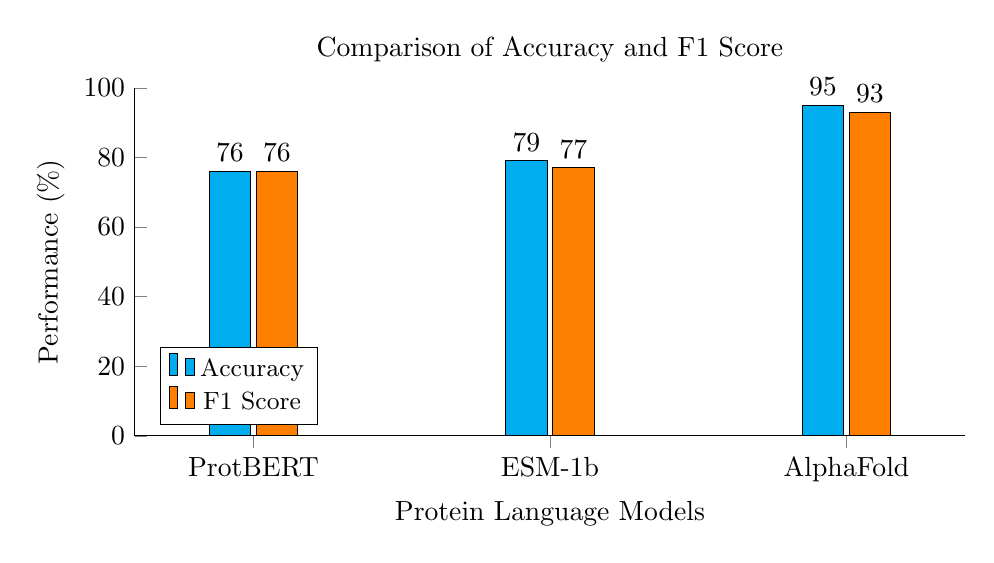
\begin{tikzpicture}
\begin{axis}[
    width=\textwidth, height=6cm,
    ybar,
    bar width=15pt,
    symbolic x coords={ProtBERT, ESM-1b, AlphaFold},
    xtick=data,
    nodes near coords,
    nodes near coords align={vertical},
    ymin=0, ymax=100,
    ylabel={Performance (\%)},
    xlabel={Protein Language Models},
    legend pos=south west,
    legend style={font=\small},
    title={Comparison of Accuracy and F1 Score},
    axis x line*=bottom,
    axis y line*=left,
    enlarge x limits=0.2
]

% Accuracy Data
\addplot[fill=cyan] coordinates {
    (ProtBERT, 76)   % ProtBERT subcellular localization
    (ESM-1b, 79)     % ESM-1b subcellular localization
    (AlphaFold, 95)    % AlphaFold fold prediction (general metric)
};

% F1 Score Data
\addplot[fill=orange] coordinates {
    (ProtBERT, 76)   % ProtBERT subcellular localization
    (ESM-1b, 77)     % ESM-1b subcellular localization
    (AlphaFold, 93)    % AlphaFold fold classification
};

\legend{Accuracy, F1 Score}
\end{axis}
\end{tikzpicture}

\end{frame}


\begin{frame}{Applications of Protein Language Models}
    \begin{tikzpicture}
        % Nodes for Applications
        \node (a1) [draw, rounded corners, fill=blue!20, text centered, minimum width=3cm, minimum height=1cm] at (0,-2) {Protein Structure Prediction};
        \node (a2) [draw, rounded corners, fill=green!20, text centered, minimum width=3cm, minimum height=1cm] at (6,0) {Drug Discovery};
        \node (a3) [draw, rounded corners, fill=orange!20, text centered, minimum width=3cm, minimum height=1cm] at (6,-2) {Disease Understanding};
        \node (a4) [draw, rounded corners, fill=purple!20, text centered, minimum width=3cm, minimum height=1cm] at (6,-4) {Synthetic Biology};

        % Arrows between the applications
        \pause
        \draw[->, thick] (a1) -- (a2);
        \draw[->, thick] (a1) -- (a3);
        \draw[->, thick] (a1) -- (a4);
        
        % Add small icons for each application
        \node at (-2,-1.3) {\includegraphics[width=0.8cm]{images/protein.PNG}}; % Protein structure icon
        \node at (7,0.7) {\includegraphics[width=0.8cm]{images/pill.PNG}}; % Drug discovery icon
        \node at (7.5,-1.3) {\includegraphics[width=0.8cm]{images/microscope.PNG}}; % Disease icon
        \node at (7,-3.3) {\includegraphics[width=0.8cm]{images/testtube.PNG}}; % Synthetic biology icon
    \end{tikzpicture}
\end{frame}

\begin{frame}{Challenges of Protein Language Models}
    \begin{tikzpicture}[
        node distance=1.5cm,
        challenge/.style={draw, shading=axis, left color=blue!50, right color=cyan!30, text centered, rounded corners, minimum height=1cm, minimum width=2.5cm},
        subchallenge/.style={draw, shading=axis, left color=blue!30, right color=purple!30, text centered, rounded corners, minimum height=1cm, minimum width=2.5cm}
    ]
        
        % Central Node (Challenges)
        \node[challenge, align = center, xshift = -1cm] (challenges) {Challenges};
        
        % First level nodes
        \node[subchallenge, below right=of challenges] (data) {Data Limitations};
        \node[subchallenge, below left=of challenges] (computational) {Computational Cost};
        \node[subchallenge, below=of challenges] (biological) {Biological Interpretation};
        
        \draw[->] (challenges.south) -- (data);
        \draw[->] (challenges.south) -- (computational);
        \draw[->] (challenges.south) -- (biological);

        % Sub-nodes for Computational Cost with Image
        \pause
        \node[below=0.3cm of computational] (computational-img1) {\includegraphics[width=1.5cm]{images/computational.png}};
        \node[subchallenge, below=0.3cm of computational-img1] {High Processing Power};
        \node[subchallenge, below=1.5cm of computational-img1] {Expensive Resources};

        % Sub-nodes for Biological Interpretation with Image
        \pause
        \node[below=0.3cm of biological] (biological-img1) {\includegraphics[width=1.5cm]{images/biological.png}};
        \node[subchallenge, below=0.3cm of biological-img1] {Hard to Translate};
        \node[subchallenge, below=1.5cm of biological-img1] {Complex Biological Context};

        % Sub-nodes for Data Limitations with Image
        \pause
        \node[below=0.3cm of data] (data-img1) {\includegraphics[width=1.5cm]{images/db.png}};
        \node[subchallenge, below=0.3cm of data-img1] {Limited Datasets};
        \node[subchallenge, below=1.5cm of data-img1] {Lack of Data};


    \end{tikzpicture}
\end{frame}

\begin{frame}{Future Directions of Protein Language Models}
\setbeamercovered{transparent}
    \begin{columns}
        % Left Column: Tasks
        \column{0.45\textwidth}

        \begin{center}
            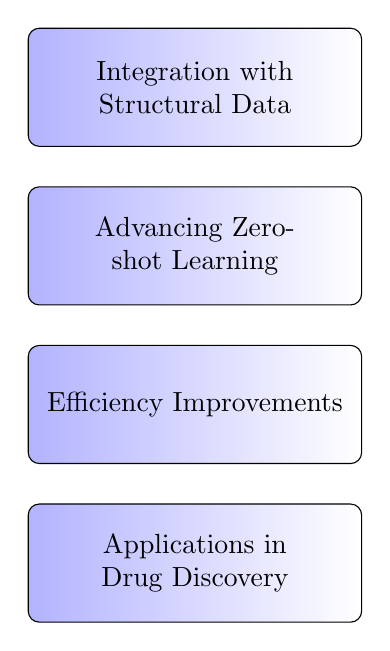
\begin{tikzpicture}[
                node distance=0.3cm and 1.2cm,
                align=center,
                rounded corners,
                every node/.style={},
                input/.style={draw,  shading=axis, left color=blue!30, right color=white!30, text width=4cm, minimum height=1.5cm},
                arrow/.style={-Stealth, thick},
                scale=0.8
            ]

            % Tasks
            {\node[input, opacity=1] (structure) {Integration with Structural Data};}
            \pause
            {\node[input, below=0.5cm of structure, opacity=1] (interactions) {Advancing Zero-shot Learning};}
            \pause
            {\node[input, below=0.5cm of interactions, opacity=1] (mutation) {Efficiency Improvements};}
            \pause
            {\node[input, below=0.5cm of mutation, opacity=1]{Applications in Drug Discovery};}

        \end{tikzpicture}
        \end{center}

        % Right Column: Models
        \column{0.55\textwidth}
        \begin{center}
            \begin{tikzpicture}[
                node distance=0.3cm and 1,
                align=center,
                rounded corners,
                every node/.style={},
                input/.style={draw, fill=greyblue!40, text width=4cm, minimum height=.8cm},
                output/.style={draw,fill=white!10, text width=5cm, minimum height=.8cm},
                arrow/.style={-Stealth, thick},
                scale=0.8
            ]
            \only<1>{
                % \node {\includegraphics[width=\textwidth]{images/stdetr.png}};
                \node[](alpic) at (0,3.5) {\includegraphics[width=5cm, keepaspectratio]{images/structural_data.PNG}};
            }
             \only<2>{
                \node[](pipic) at (0,3.5) {\includegraphics[width=5cm, keepaspectratio]{images/zero_shot_learning.PNG}};
            }
            \only<3>{
               \node[] (mutpic) at (0,3.5) {\includegraphics[width=5cm, keepaspectratio]{images/efficiency.PNG}};
            }

            \only<4>{
                \node[] (mutpic) at (0,3.5) {\includegraphics[width=5cm, keepaspectratio]{images/drug_discovery.PNG}};
            }
            

        \end{tikzpicture}
        \end{center}
    \end{columns}
\end{frame}




\begin{frame}{Conclusion}
    \begin{columns}
        % Left column with pictures
        \begin{column}{0.5\textwidth}
            \centering
            \includegraphics[width=0.7\textwidth]{images/conclusion.PNG} 
        \end{column}
        
        % Right column with brief text
        \begin{column}{0.5\textwidth}
            \begin{itemize}
            \item Powerful tools for protein sequence analysis.
            \item Enable insights into protein structures and functions.
            \item Revolutionizing drug design and bioinformatics.
        \end{itemize}
        \end{column}
    \end{columns}
\end{frame}




\end{document}
